\label{capitolo3}
\section{Modelli a blocchi e ad oggetti}
Per identificare dei modelli o dei parametri a volte ci affidiamo a delle simulazioni di modelli che possono essere di due tipi:
\begin{itemize}
\item Orientati ai blocchi
\item Orientati agli oggetti
\end{itemize}
Nel caso di modelli orientati ai blocchi l'ordinamento � di tipo \emph{causale} ovvero un blocco ha un ingresso ed un uscita e un uscita pu� connettersi a uno o pi� ingressi attraverso connessioni \emph{input/output}.
Nel caso di modelli orientati agli oggetti abbiamo una \emph{a-causalit�} tra i vari oggetti; le connessioni tra i vari oggetti avvengono attraverso delle porte che instaurano un collegamento di uguaglianza tra ci� che viene collegato.
Vediamo ora attraverso un esempio la differenza tra modelli BO e OO.
\subsection{Legge di Ohm}
\subsubsection{Caso BO}
Se voglio modellizzare un resistore collegato ad un generatore dovr� costruire due modelli, uno nel caso in cui il generatore � un generatore di tensione, in questo caso il modello � dato da:
$$
\begin{array}{ccc}
V&=&E\\
I&=&V/R
\end{array}
$$
Nel caso in cui invece il generatore fornisca una corrente il modello diventa:
$$
\begin{array}{ccc}
I&=&A\\
V&=&RI
\end{array}
$$
Per gli stessi componenti abbiamo dovuto definire due differenti condizioni limite e \emph{due modelli differenti}.
\subsubsection{Caso OO}
Nel caso di modelli orientati agli oggetti opto per un differente approccio; prima di tutto diamo una definizione di \emph{porte}: esse possono essere definite come quei terminali fisici che interfacciano il componente con il mondo esterno. Nel caso del resistore sono i due pin di connessione. Il modello del resistore diventa quello identificato nell'equazione \ref{res}
\begin{equation}
\label{res}
RES:
\left\{
\begin{array}{ccc}
a.I+b.I&=&0\\
a.V-b.V&=&R a.I
\end{array}
\right .
\end{equation}
Introduciamo poi i due generatori rispettivamente quello di tensione \ref{vgen} e quello di corrente \ref{cgen} ed inoltre la massa \ref{gnd}
\begin{equation}
\label{vgen}
VGEN:
\left\{
\begin{array}{ccc}
a.I+b.I&=&0\\
a.V-b.V&=&R E
\end{array}
\right.
\end{equation}
\begin{equation}
\label{cgen}
CGEN:
\left\{
\begin{array}{ccc}
a.I+b.I&=&0\\
a.I&=&-A
\end{array}
\right.
\end{equation}
\begin{equation}
\label{gnd}
GND:\quad a.V=0
\end{equation}
\begin{figure}
\centering
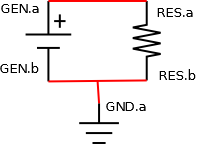
\includegraphics[width=5cm]{img/circuito.png}
\caption{Schema del circuito in rosso le connessioni\label{fig:circuito}}
\end{figure}
Cosi facendo vediamo come i due modelli descritti prima attraverso il sistema BO in questo caso possano essere descritti semplicemente cambiano il \emph{"modulo"} generatore; ovvero interscambiando le equazioni che descrivono i due generatori.\\
Bisogna per� descrivere le equazioni che governano le connessioni (Fig. \ref{fig:circuito}), che anche in questo caso sono comuni per i due tipi di generatori.\\
\begin{eqnarray}
GEN.a.V &=& RES.a.V\\
GEN.a.I + RES.a.I &=& 0\\
GEN.b.V &=& GND.a.V\\
RES.b.V &=& GND.a.V\\
GEN.b.I + RES.b.I + GND.a.I &=& 0
\end{eqnarray}
Le variabili che caratterizzano una porta possono essere di due tipi:
\begin{itemize}
\item variabili di \emph{effort} ovvero variabili che sono definite attraverso la differenza da un riferimento (es. ddp).
\item variabili \emph{flow} definite come un flusso attraverso un canale (es. corrente).
\end{itemize}
Per connettere N porte ho bisogno di $N-1$ equazioni per ogni variabile di effort ed una sola per tutte le variabili di flusso.\\
Come si � visto entrambi i metodi di modellizzazione incapsulano il comportamento del modello esponendo un'interfaccia, questo per ragioni di scalabilit�. I modelli BO richiedono per� che il sistema sia orientato cio� richiede che le variabili di ingresso e uscita siano ben specificate per ogni blocco. Nei modelli OO, invece, non � richiesto che i componenti siano orientati.

\subsection{Concetto di circuito elettrico equivalente}
Nei modelli OO le porte sono naturalmente associate ad un trasferimento di energia. Ad esempio consideriamo una porta con un unica variabile di flusso e una di effort in diversi casi:
\begin{itemize}
\item elettrico (tensione v e corrente i): vi = potenza
\item meccanico translazionale (posizione x e forza f): $\dot{x}$f = potenza
\item meccanico rotazionale (angolo $\theta$ fozta $\tau$): $\dot{\theta}\tau$ = potenza
\item termico (temperatura T e potenza Q): in questo caso la potenza non � il prodotto delle due
\end{itemize}
L'equivalente elettrico � utile anche per descrivere quei fenomeni legati all'energia; come nel caso in cui:
\begin{itemize}
\item l'accumulo di energia � legato a una variabile di effort come nel caso $E=CT$ dove $C$ � la capacit� termica.
\item il trasferimento di energia � legato linearmente a una differenza di variabili $Q=G\Delta T$ dove $G$ � la conduttanza termica.
\end{itemize}
